\documentclass[twocolumn, 11pt]{article}%
\usepackage{amsmath, amssymb, esint, gensymb, hyperref, mathtools}
\usepackage{graphicx, cuted, geometry, float, scalerel, xcolor, xfrac}

\newcommand\sbullet[1][.5]{\mathbin{\ThisStyle{\vcenter{\hbox{%
  \scalebox{#1}{$\SavedStyle\bullet$}}}}}%
}

\geometry{
    a4paper,
    total={170mm,260mm},
}

\begin{document}

\begin{strip}
  \vspace*{\dimexpr-\stripsep}
  \begin{center}
      \Large\textbf{FISIKA 2}\\
      \large{Pertemuan 1 - Minggu 9 (306344)}\\
      \large{\today}
   \end{center}
\end{strip}

\section{Medan Listrik}
\subsection{Asal Muasal Medan Magnet}%
    Yang perlu diperhatikan adalah tidak adanya muatan Magnetik, atau
    tidak ada magnet monopole. Jika magnet permanen dipotong maka tiap
    potongan tetap merupakan magnet dipole, yaitu kutub utara dan kutub
    selatan SELALU berpasangan.
    \begin{center}
        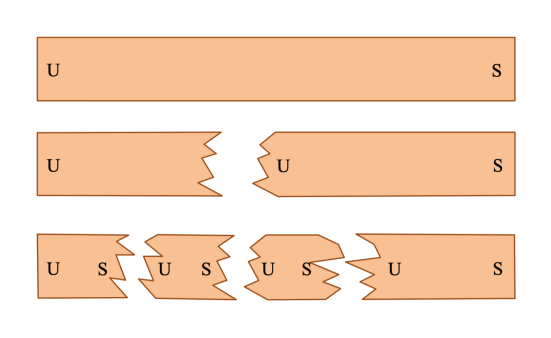
\includegraphics[width=150px]{1.png}
    \end{center}

    Pada magnet, kutub yang berlawanan saling tolak menolak. Kutub yang
    sejenis jika didekatkan, maka akan terjadi gaya tarik-menarik.

    \begin{center}
        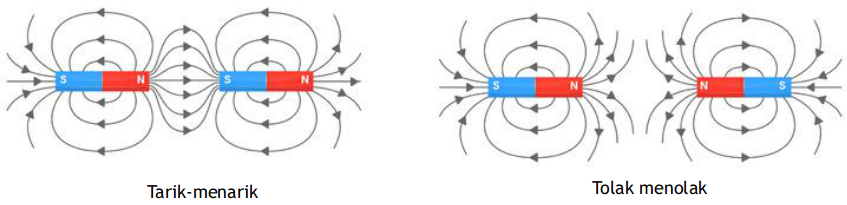
\includegraphics[width=220px]{2.png}
    \end{center}

    Cara memperoleh medan magnet adalah dari material Magnet (besi,
    nikel) dan juga dari muatan listrik yang bergerak. Pada kasus medan
    magnetik dari arus listrik yang bergerak, digunakan aturan tangan
    kanan untuk memudahkan kita menentukan arah vektor induksi magnet
    ($\vec B$) dari arah arus listrik yang diketahui, begitupun
    sebaliknya.

    \begin{center}
        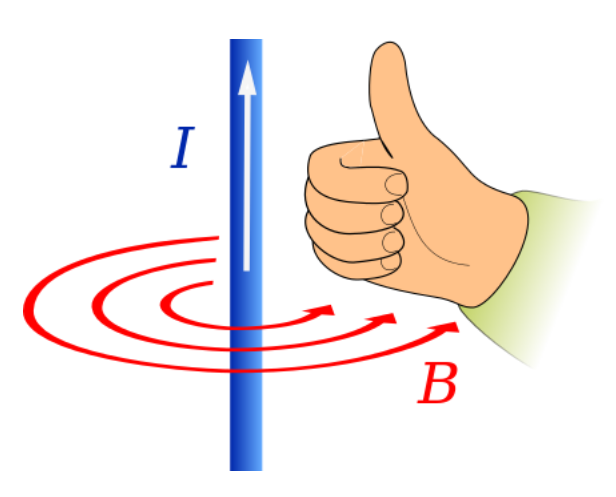
\includegraphics[width=150px]{3.png}
    \end{center}

\subsection{Medan Magnet (Vektor Induksi Magnet $\vec B$)}%
    Medan Magnet adalah besaran vektor dengan satuan \textbf{Weber/$m^2$
    (W/$m^2$)}, atau Tesla (T).

    \begin{center}
    1 T = 1 W/$m^2$ = $10^4$ G
    \end{center}

\subsection{Garis Gaya Magnet}%
Garis gaya magnet dilukiskan keluar dari kutub utara dan masuk di kutub selatan.

Kerapatan garis gaya per satuan luas di suatu titik menggambarkan kekuatan medan magnet di titik tersebut.

Kerapatan garis gaya terbesar diamati di kutub magnet. Ini berarti medan magnet paling kuat di daerah kutub.

Makin jauh dari kutub maka makin kecil kerapatan garis gaya. Ini berarti makin jauh dari kutub maka makin lemah medan magnet.

\begin{center}
    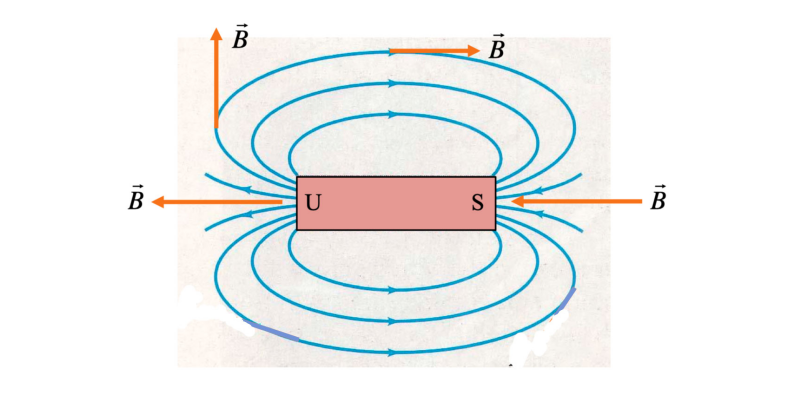
\includegraphics[width=180px]{4.png}
\end{center}

Besar medan Magnet $\alpha$ kerapatan garis gaya magnet. Atau, besar medan magnet sebanding dengan kerapatan garis gaya magnet.

\subsection{Gaya Magnet ($\overrightarrow{F_B}$)}%

\begin{center}
    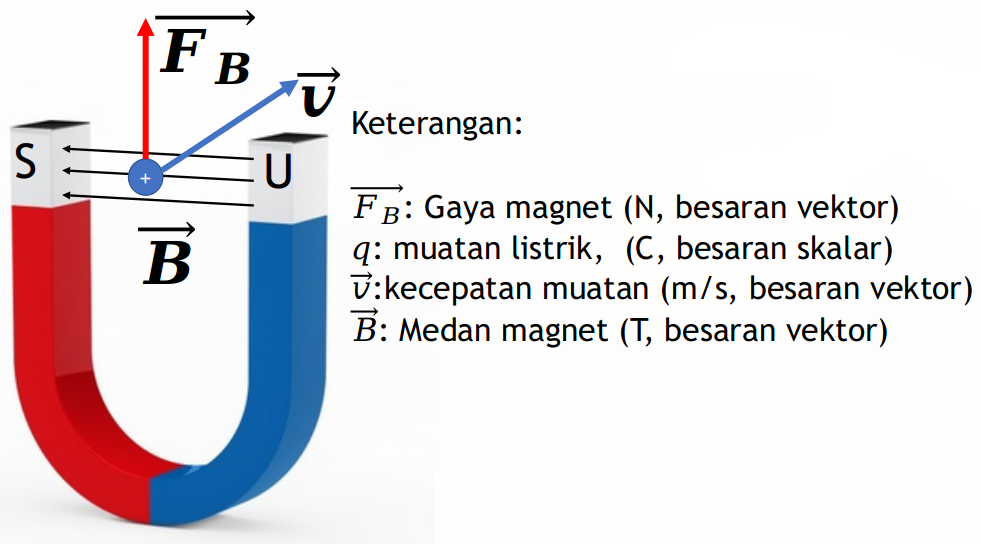
\includegraphics[width=220px]{5.png}
\end{center}

Arah gaya magnet bisa dibantu dengan aturan tangan kanan.
\begin{center}
    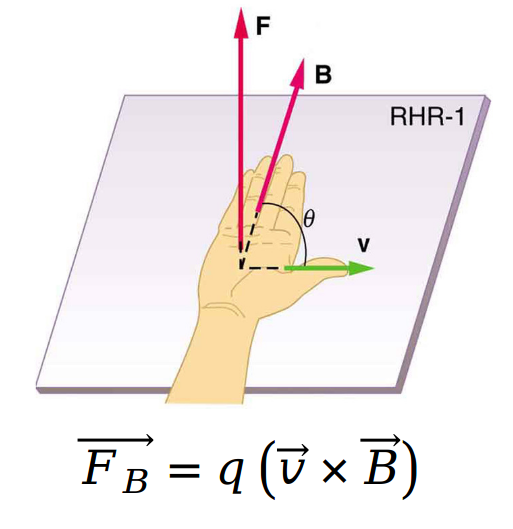
\includegraphics[width=100px]{6.png}
\end{center}

di mana $\overrightarrow{F_B}$ tegak lurus dengan bidang $\vec V$ dan
$\vec B$. Dengan rumus perkalian cross vektor Fisdas 1, didapatkan bahwa 

\[ \overrightarrow{F_B} = q[(v_y B_z - v_z B_y)\hat i + (v_z B_x - v_x
B_z)\hat j + (v_x B_y - v_y B_x)\hat k] \]

Perlu diingat di sini bahwa V dan B tidak harus tegak lurus 90\textdegree.

\subsection{Gerak Muatan Dalam Medan Magnet Yang Seragam}%
Dapat terjadi 3 macam gerak pada kasus ini, yaitu
\begin{enumerate}
    \item Gerak Lurus
    \item Gerak Melingkar
    \item Gerak Spiral, gabungan dari gerak lurus dan gerak melingkar.
\end{enumerate}

\subsubsection{Gerak Lurus}%
\begin{center}
    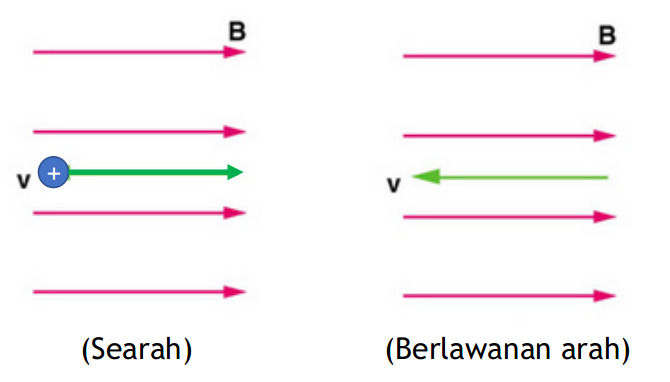
\includegraphics[width=200px]{7.png}
\end{center}

Gerak lurus yang dimaksudkan di sini adalah muatan bergerak lurus
(kecepatan sama) karena tidak mendapatkan Gaya Magnetik.

$\vec v$ dan $\vec B$ paralel (searah) atau $\vec v$ dan $\vec B$
antiparalel (berlawanan arah)

Dalam bahasa matematika $\theta = 0\degree$ yang disebut paralel dan
$\theta = 180\degree$ yang disebut berlawanan arah. Bisa kita lihat bahwa

\[ \sin 0\degree = 0\]
\[ \sin 180\degree = 0\]

Maka didapat bahwa besar Gaya Magnet
\begin{align*}
    F_B &= qvB\sin\theta\\
        &= 0
\end{align*}

\subsubsection{Gerak Melingkar}%
Gerak melingkar terjadi ketika $\vec v$ dan $\vec B$ tegak lurus dan
memiliki besar sudut $\theta=90\degree$. Diketahui bahwa $\sin
90\degree=1$. Maka besar gaya magnetnya adalah
\begin{align*}
    F_B &= qvB\sin\theta\\
        &= qvB
\end{align*}

\begin{center}
    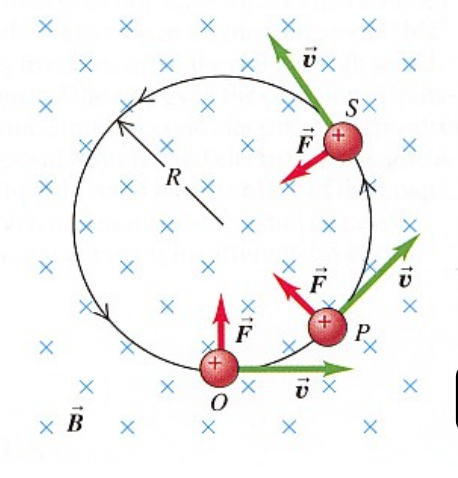
\includegraphics[width=100px]{8.png}
\end{center}

Di sini gaya magnet menjadi gaya sentripetal yang menyebabkan muatan
bergerak melingkar. Arah $\vec B$ masuk ke dalam kertas dan dilambangkan
dengan $\times$.

\begin{center}
    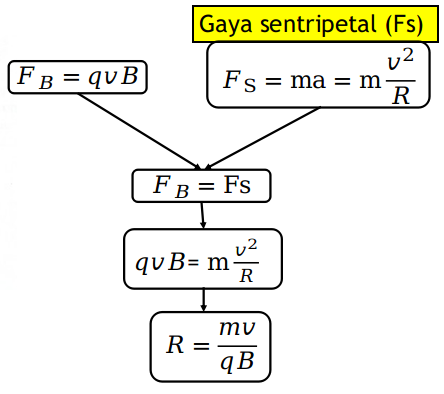
\includegraphics[width=160px]{9.png}
\end{center}

\subsubsection{Gerak Spiral}%
\begin{center}
    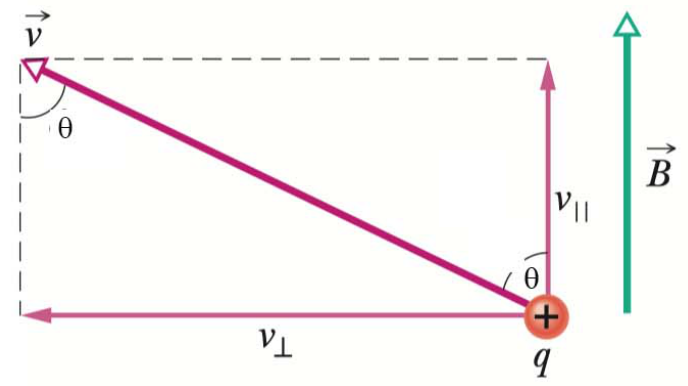
\includegraphics[width=200px]{10.png}
\end{center}

Gerak spiral terjadi karena $\vec B$ dan $\vec v$ mempunyai sudut 
$\theta$ seperti gambar di atas. Sehingga

\[v_{\parallel} =v\cos\theta \]
\[v_{\perp} =v\sin\theta \]

Dan arah gaya magnetnya menuju ke dalam kertas ($\times$)

Karena $v_{\parallel}$ sejajar dengan $\vec B$, maka akan menghasilkan
gerak lurus (dikarenakan tidak adanya gaya magnet). Sedangkan karena
$v_{\perp}$ sejajar dengan $\vec B$, maka akan menghasilkan Gaya Magnet
dengan arah masuk ke dalam kertas, yang menyebabkan gerak melingkar. Dan
karena kedua gerak tersebut dilakukan pada satu muatan (digabung) maka
terjadilah gerak spiral.

\begin{center}
    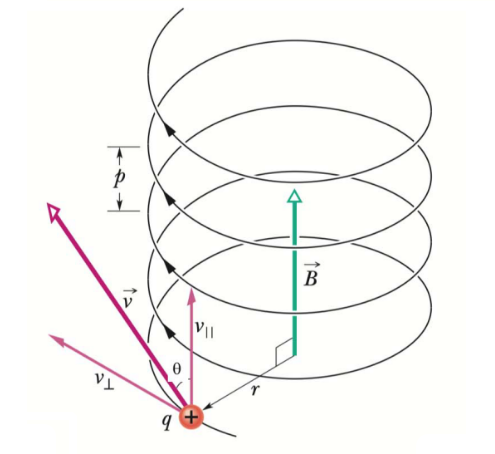
\includegraphics[width=140px]{11.png}
\end{center}

\subsection{Gaya Magnet Pada Kawat Arus Dalam Medan Magnet}%
\begin{center}
    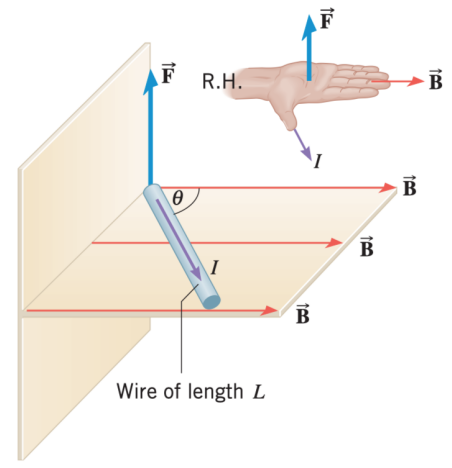
\includegraphics[width=150px]{12.png}
\end{center}
Sebelumnya diketahui bahwa Besar gaya magnet pada muatan tunggal ($q$)
adalah
\[ F_B = qvB\sin\theta \]

Maka, Besar gaya magnet pada banyak muatan (dengan arus I) adalah
\[ F_B = \Delta qvB\sin\theta.\frac{\Delta t}{\Delta t} \]

Sehingga,
\[ F_B = \left(\frac{\Delta q}{\Delta t}\right)(v\Delta T)B\sin\theta \]

karena $\displaystyle \frac{\Delta q}{\Delta t}=I$ dan $v\Delta T=L$,
maka

\[ F_B = ILB\sin\theta \]

dan

\[ \overrightarrow{F_B} = I(\vec L\times\vec B) \]

\end{document}
